%% Aide-mémoire
\documentclass[french, landscape]{article}
%% -----------------------------
%% Préambule
%% -----------------------------
% !TEX encoding = UTF-8 Unicode
% LaTeX Preamble for all cheatsheets
% Author : Gabriel Crépeault-Cauchon

% HOW-TO : copy-paste this file in the same directory as your .tex file, and add in your preamble the next command right after you have specified your documentclass : 
% \input{preamble-cheatsht.tex}
% ---------------------------------------------
% ---------------------------------------------

% Extra note : this preamble creates document that are meant to be used inside the multicols environment. See the documentation on internet for further information.

%% -----------------------------
%% Encoding packages
%% -----------------------------
\usepackage[utf8]{inputenc}
\usepackage[T1]{fontenc}
\usepackage{babel}
\usepackage{lmodern}

%% -----------------------------
%% Variable definition
%% -----------------------------
\def\auteur{Gabriel Crépeault-Cauchon / Nicholas Langevin}
\def\BackgroundColor{white}

%% -----------------------------
%% Margin and layout
%% -----------------------------
% Determine the margin for cheatsheet
\usepackage[landscape, hmargin=1cm, vmargin=1.7cm]{geometry}
\usepackage{multicol}

% Remove automatic indentation after section/subsection title.
\setlength{\parindent}{0cm}

% Save space in cheatsheet by removing space between align environment and normal text.
\usepackage{etoolbox}
\newcommand{\zerodisplayskips}{%
  \setlength{\abovedisplayskip}{0pt}%
  \setlength{\belowdisplayskip}{0pt}%
  \setlength{\abovedisplayshortskip}{0pt}%
  \setlength{\belowdisplayshortskip}{0pt}}
\appto{\normalsize}{\zerodisplayskips}
\appto{\small}{\zerodisplayskips}
\appto{\footnotesize}{\zerodisplayskips}

%% -----------------------------
%% URL and links
%% -----------------------------
\usepackage{hyperref}
\hypersetup{colorlinks = true, urlcolor = gray!70!white, linkcolor = black}

%% -----------------------------
%% Document policy (uncomment only one)
%% -----------------------------
%	\usepackage{concrete}
	\usepackage{mathpazo}
%	\usepackage{frcursive} %% permet d'écrire en lettres attachées
%	\usepackage{aeguill}
%	\usepackage{mathptmx}
%	\usepackage{fourier} 

%% -----------------------------
%% Math configuration
%% -----------------------------
\usepackage[fleqn]{amsmath}
\usepackage{amsthm,amssymb,latexsym,amsfonts}
\usepackage{empheq}
\usepackage{numprint}
\usepackage{dsfont} % Pour avoir le symbole du domaine Z

% Mathematics shortcuts

\newcommand{\reels}{\mathbb{R}}
\newcommand{\entiers}{\mathbb{Z}}
\newcommand{\naturels}{\mathbb{N}}
\newcommand{\eval}{\biggr \rvert}
\usepackage{cancel}
\newcommand{\derivee}[1]{\frac{\partial}{\partial #1}}
\newcommand{\prob}[1]{\Pr \left( #1 \right)}
\newcommand{\esp}[1]{\mathrm{E} \left[ #1 \right]} % espérance
\newcommand{\variance}[1]{\mathrm{Var} \left( #1   \right)}
\newcommand{\covar}[1]{\mathrm{Cov} \left( #1   \right)}
\newcommand{\laplace}{\mathcal{L}}
\newcommand{\deriv}[2][]{\frac{\partial^{#1}}{\partial #2^{#1}}}
\newcommand{\e}[1]{\mathrm{e}^{#1}}
\newcommand{\te}[1]{\text{exp}\left\{#1\right\}}
\DeclareMathSymbol{\shortminus}{\mathbin}{AMSa}{"39}



% To indicate equation number on a specific line in align environment
\newcommand\numberthis{\addtocounter{equation}{1}\tag{\theequation}}

%
% Actuarial notation packages
%
\usepackage{actuarialsymbol}
\usepackage{actuarialangle}

%
% Matrix notation for math symbols (\bm{•})
%
\usepackage{bm}
% Matrix notation variable (bold style)
\newcommand{\matr}[1]{\mathbf{#1}}



%% -----------------------------
%% tcolorbox configuration
%% -----------------------------
\usepackage[most]{tcolorbox}
\tcbuselibrary{xparse}
\tcbuselibrary{breakable}

%%
%% Coloured box "definition" for definitions
%%
\DeclareTColorBox{definition}{ o }				% #1 parameter
{
	colframe=blue!60!green,colback=blue!5!white, % color of the box
	breakable, 
	pad at break* = 0mm, 						% to split the box
	title = {#1},
	after title = {\large \hfill \faBook},
}
%%
%% Coloured box "definition2" for definitions
%%
\DeclareTColorBox{definitionNOHFILL}{ o }				% #1 parameter
{
	colframe=blue!60!green,colback=blue!5!white, % color of the box
	pad at break* = 0mm, 						% to split the box
	title = {#1},
	before title = {\faBook \quad },
	breakable
}


%%
%% Coloured box "algo" for algorithms
%%
\newtcolorbox{algo}[ 1 ]
{
	colback = blue!5!white,
	colframe = blue!75!black,
	title=#1,
	fonttitle = \bfseries,
	breakable
}
%%
%% Coloured box "conceptgen" for points adding to a concept's deifintion
%%
\newtcolorbox{conceptgen}[ 1 ]
{
	breakable,
	colback = beaublue,
	colframe = airforceblue,
	title=#1,
	fonttitle = \bfseries
}
%%
%% Coloured box "probch3" pour formules relatives au 3ème chapitre de prob
%%
\newtcolorbox{probch3}[ 1 ]
{
	colback = ruddypink,
	colframe = burgundy,
	fonttitle = \bfseries,	
	breakable,
	title=#1
}
%%
%% Coloured box "formula" for formulas
%%
\newtcolorbox{formula}[ 1 ]
{
	colback = green!5!white,
	colframe = green!70!black,
	breakable,
	fonttitle = \bfseries,
	title=#1
}
%%
%% Coloured box "formula" for formulas
%%
\DeclareTColorBox{algo2}{ o }
{
	enhanced,
	title = #1,
	colback=blue!5!white,	
	colbacktitle=blue!75!black,
	fonttitle = \bfseries,
	breakable,
	boxed title style={size=small,colframe=arsenic} ,
	attach boxed title to top center = {yshift=-3mm,yshifttext=-1mm},
}
%%
%% Coloured box "examplebox" for formulas
%%
\newtcolorbox{examplebox}[ 1 ]
{
	colback = lightmauve,
	colframe = antiquefuchsia,
	breakable,
	fonttitle = \bfseries,title=#1
}
%%
%% Coloured box "rappel" pour rappel de formules
%%
\newtcolorbox{rappel}[ 1 ]
{
	colback = ashgrey,
	colframe = arsenic,
	breakable,
	fonttitle = \bfseries,title=#1
}
%%
%% Coloured box "rappel" pour rappel de formules
%%
\DeclareTColorBox{rappel_enhanced}{ o }
{
	enhanced,
	title = #1,
	colback=ashgrey, % color of the box
%	colframe=blue(pigment),
%	colframe=arsenic,	
	colbacktitle=arsenic,
	fonttitle = \bfseries,
	breakable,
	boxed title style={size=small,colframe=arsenic} ,
	attach boxed title to top center = {yshift=-3mm,yshifttext=-1mm},
}
%%
%% Coloured box "notation" for notation and terminology
%%
\DeclareTColorBox{distributions}{ o }			% #1 parameter
{
	enhanced,
	title = #1,
	colback=gray(x11gray), % color of the box
%	colframe=blue(pigment),
	colframe=arsenic,	
	colbacktitle=aurometalsaurus,
	fonttitle = \bfseries,
	boxed title style={size=small,colframe=arsenic} ,
	attach boxed title to top center = {yshift=-3mm,yshifttext=-1mm},
	breakable
%	left=0pt,
%  	right=0pt,
%    box align=center,
%    ams align*
%  	top=-10pt
}

%% -----------------------------
%% Graphics and pictures
%% -----------------------------
\usepackage{graphicx}
\usepackage{pict2e}
\usepackage{tikz}

%% -----------------------------
%% insert pdf pages into document
%% -----------------------------
\usepackage{pdfpages}

%% -----------------------------
%% Color configuration
%% -----------------------------
\usepackage{color, soulutf8, colortbl}


%
%	Colour definitions
%
\definecolor{blue(munsell)}{rgb}{0.0, 0.5, 0.69}
\definecolor{blue(matcha)}{rgb}{0.596, 0.819, 1.00}
\definecolor{blue(munsell)-light}{rgb}{0.5, 0.8, 0.9}
\definecolor{bleudefrance}{rgb}{0.19, 0.55, 0.91}
\definecolor{blizzardblue}{rgb}{0.67, 0.9, 0.93}
\definecolor{bondiblue}{rgb}{0.0, 0.58, 0.71}
\definecolor{blue(pigment)}{rgb}{0.2, 0.2, 0.6}
\definecolor{bluebell}{rgb}{0.64, 0.64, 0.82}
\definecolor{airforceblue}{rgb}{0.36, 0.54, 0.66}
\definecolor{beaublue}{rgb}{0.74, 0.83, 0.9}
\definecolor{cobalt}{rgb}{0.0, 0.28, 0.67}	% nice light blue-ish
\definecolor{blue_rectangle}{RGB}{83, 84, 244}		% ACT-2004
\definecolor{indigo(web)}{rgb}{0.29, 0.0, 0.51}	% purple-ish
\definecolor{antiquefuchsia}{rgb}{0.57, 0.36, 0.51}	%	pastel dark purple ish
\definecolor{darkpastelpurple}{rgb}{0.59, 0.44, 0.84}
\definecolor{gray(x11gray)}{rgb}{0.75, 0.75, 0.75}
\definecolor{aurometalsaurus}{rgb}{0.43, 0.5, 0.5}
\definecolor{ruddypink}{rgb}{0.88, 0.56, 0.59}
\definecolor{pastelred}{rgb}{1.0, 0.41, 0.38}		
\definecolor{lightmauve}{rgb}{0.86, 0.82, 1.0}
\definecolor{azure(colorwheel)}{rgb}{0.0, 0.5, 1.0}
\definecolor{darkgreen}{rgb}{0.0, 0.2, 0.13}			
\definecolor{burntorange}{rgb}{0.8, 0.33, 0.0}		
\definecolor{burntsienna}{rgb}{0.91, 0.45, 0.32}		
\definecolor{ao(english)}{rgb}{0.0, 0.5, 0.0}		% ACT-2003
\definecolor{amber(sae/ece)}{rgb}{1.0, 0.49, 0.0} 	% ACT-2004
\definecolor{green_rectangle}{RGB}{131, 176, 84}		% ACT-2004
\definecolor{red_rectangle}{RGB}{241,112,113}		% ACT-2004
\definecolor{amethyst}{rgb}{0.6, 0.4, 0.8}
\definecolor{amethyst-light}{rgb}{0.6, 0.4, 0.8}
\definecolor{ashgrey}{rgb}{0.7, 0.75, 0.71}			% dark grey-black-ish
\definecolor{arsenic}{rgb}{0.23, 0.27, 0.29}			% light green-beige-ish gray
\definecolor{amaranth}{rgb}{0.9, 0.17, 0.31}
\definecolor{brickred}{rgb}{0.8, 0.25, 0.33}
\definecolor{pastelred}{rgb}{1.0, 0.41, 0.38}

%
% Useful shortcuts for coloured text
%
\newcommand{\orange}{\textcolor{orange}}
\newcommand{\red}{\textcolor{red}}
\newcommand{\cyan}{\textcolor{cyan}}
\newcommand{\blue}{\textcolor{blue}}
\newcommand{\green}{\textcolor{green}}
\newcommand{\purple}{\textcolor{magenta}}
\newcommand{\yellow}{\textcolor{yellow}}

%% -----------------------------
%% Enumerate environment configuration
%% -----------------------------
%
% Custum enumerate & itemize Package
%
\usepackage{enumitem}
%
% French Setup for itemize function
%
\frenchbsetup{StandardItemLabels=true}
%
% Change default label for itemize
%
\renewcommand{\labelitemi}{\faAngleRight}


%% -----------------------------
%% Tabular column type configuration
%% -----------------------------
\newcolumntype{C}{>{$}c<{$}} % math-mode version of "l" column type
\newcolumntype{L}{>{$}l<{$}} % math-mode version of "l" column type
\newcolumntype{R}{>{$}r<{$}} % math-mode version of "l" column type
\newcolumntype{f}{>{\columncolor{green!20!white}}p{1cm}}
\newcolumntype{g}{>{\columncolor{green!40!white}}m{1.2cm}}
\newcolumntype{a}{>{\columncolor{red!20!white}$}p{2cm}<{$}}	% ACT-2005
% configuration to force a line break within a single cell
\usepackage{makecell}


%% -----------------------------
%% Fontawesome for special symbols
%% -----------------------------
\usepackage{fontawesome}

%% -----------------------------
%% Section Font customization
%% -----------------------------
\usepackage{sectsty}
\sectionfont{\color{\SectionColor}}
\subsectionfont{\color{\SubSectionColor}}

%% -----------------------------
%% Footer/Header Customization
%% -----------------------------
\usepackage{lastpage}
\usepackage{fancyhdr}
\pagestyle{fancy}

%
% Header
%
\fancyhead{} 	% Reset
\fancyhead[L]{Aide-mémoire pour~ \cours ~(\textbf{\sigle})}
\fancyhead[R]{\auteur}

%
% Footer
%
\fancyfoot{}		% Reset
\fancyfoot[R]{\thepage ~de~ \pageref{LastPage}}
\fancyfoot[L]{\href{https://github.com/ressources-act/Guide_de_survie_en_actuariat}{\faGithub \ ressources-act/Guide de survie en actuariat}}
%
% Page background color
%
\pagecolor{\BackgroundColor}




%% END OF PREAMBLE
% ---------------------------------------------
% ---------------------------------------------
%% -----------------------------
%% Variable definition
%% -----------------------------
\def\cours{Mathématiques actuarielles IARD1}
\def\sigle{ACT-2005}
\def\SectionColor{red!80!white}
\def\SubSectionColor{red!30!black}
%% -----------------------------
%% Début du document
%% -----------------------------
\begin{document}

\small
\begin{multicols*}{3} % Nombre de colonnes (peut être changé plus tard.)

\setcounter{section}{2}
\section{Estimation non-paramétrique}
\subsection*{Moments à savoir}
\begin{align*}
\mu_k^{\prime} 	& = \esp{X^k} &
\mu_k			& = \esp{(X-\mu)^k} \\
CV				& = \frac{\sigma}{\mu} \\
\text{Skewness: } \gamma			& = \frac{\mu_3}{\sigma^3}  &
\text{Kurtosis: } \kappa			& = \frac{\mu_4}{\sigma^4} \\
\end{align*}


\tikzset{every picture/.style={line width=0.75pt}} %set default line width to 0.75pt        

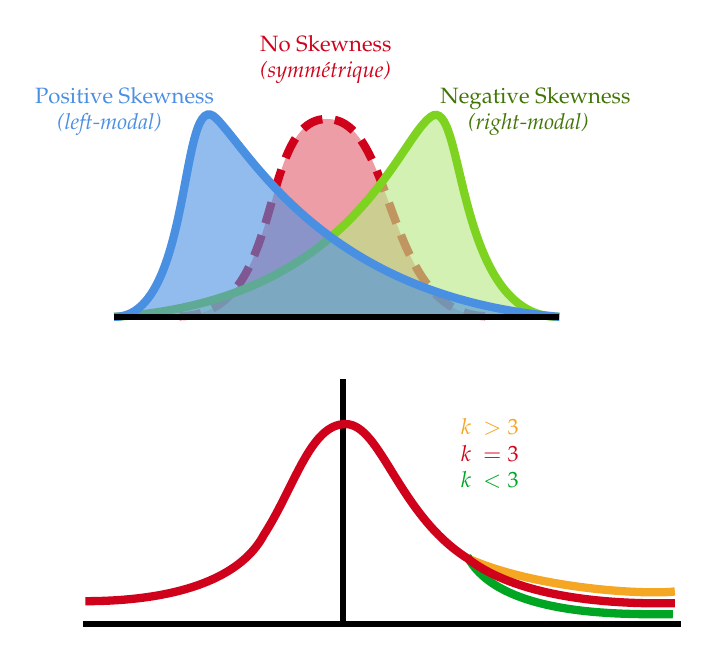
\begin{tikzpicture}[x=0.75pt,y=0.75pt,yscale=-1,xscale=1]
%uncomment if require: \path (0,300); %set diagram left start at 0, and has height of 300

%Curve Lines [id:da2688874623271533] 
\draw [color={rgb, 255:red, 208; green, 2; blue, 27 }  ,draw opacity=1 ][fill={rgb, 255:red, 208; green, 2; blue, 27 }  ,fill opacity=0.39 ][line width=3]  [dash pattern={on 7.88pt off 4.5pt}]  (80.5,138.67) .. controls (132.5,138.67) and (117.5,43.67) .. (151.5,43.67) .. controls (185.5,43.67) and (178.5,139.67) .. (229.5,138.67) ;


%Curve Lines [id:da9147539678395264] 
\draw [color={rgb, 255:red, 126; green, 211; blue, 33 }  ,draw opacity=1 ][fill={rgb, 255:red, 184; green, 233; blue, 134 }  ,fill opacity=0.64 ][line width=3]    (49,139) .. controls (163.5,131.67) and (184.83,55) .. (201.5,42.67) .. controls (218.17,30.33) and (212.5,140) .. (263.5,139) ;


%Curve Lines [id:da8124483083453555] 
\draw [color={rgb, 255:red, 74; green, 144; blue, 226 }  ,draw opacity=1 ][fill={rgb, 255:red, 74; green, 144; blue, 226 }  ,fill opacity=0.6 ][line width=3]    (49,139) .. controls (87.5,139.67) and (80.17,24.33) .. (98.5,43.67) .. controls (116.83,63) and (152.5,129.67) .. (263.5,139) ;


%Straight Lines [id:da7586443312018019] 
\draw [line width=2.25]    (49,139) -- (263.5,139) ;



%Straight Lines [id:da09355877210927566] 
\draw [line width=2.25]    (34.17,287) -- (322.17,287) ;


%Curve Lines [id:da18622021578279613] 
\draw [color={rgb, 255:red, 245; green, 166; blue, 35 }  ,draw opacity=1 ][line width=3]    (219.17,255.33) .. controls (252.17,270) and (304.17,273) .. (319.17,271.33) ;


%Curve Lines [id:da37988280307937217] 
\draw [color={rgb, 255:red, 0; green, 166; blue, 35 }  ,draw opacity=1 ][line width=3]    (219.17,254.33) .. controls (235.17,285) and (300.17,282) .. (318.17,282.33) ;


%Straight Lines [id:da5412137305076621] 
\draw [line width=2.25]    (159.17,169) -- (159.17,286) ;


%Curve Lines [id:da11948970250620294] 
\draw [color={rgb, 255:red, 208; green, 2; blue, 27 }  ,draw opacity=1 ][line width=3]    (35.17,276) .. controls (61.17,276) and (106.17,272) .. (121.17,244) .. controls (136.04,220.92) and (143.5,190.67) .. (160.5,190.67) .. controls (177.5,190.67) and (185.87,234.17) .. (219.17,255.33) .. controls (249.17,279) and (309.17,277) .. (319.17,277) ;



% Text Node
\draw (151,15) node [scale=0.8,color={rgb, 255:red, 208; green, 2; blue, 27 }  ,opacity=1 ] [align=left] {No Skewness\\\textit{(symmétrique)}};
% Text Node
\draw (252,40) node [scale=0.8,color={rgb, 255:red, 65; green, 117; blue, 5 }  ,opacity=1 ] [align=left] {Negative Skewness\\\textit{ \ \ \ \ (right-modal)}};
% Text Node
\draw (54,40) node [scale=0.8,color={rgb, 255:red, 65; green, 117; blue, 5 }  ,opacity=1 ] [align=left] {\textcolor[rgb]{0.29,0.56,0.89}{Positive Skewness}\\\textit{\textcolor[rgb]{0.29,0.56,0.89}{ \ \ \ \ (left-modal)}}};
% Text Node
\draw (230,206) node [scale=0.8,color={rgb, 255:red, 65; green, 117; blue, 5 }  ,opacity=1 ] [align=left] {$\displaystyle  \begin{array}{{>{\displaystyle}l}}
\textcolor[rgb]{0.96,0.65,0.14}{k\  >3}\\
\textcolor[rgb]{0.82,0.01,0.11}{k\ =3}\\
\textcolor[rgb]{0.0,0.65,0.14}{k\ < 3}
\end{array}$};

\end{tikzpicture}

\subsection*{3 critères pour évaluer les queues de distributions}

\begin{enumerate}

\item La loi avec le moins de moments a la queue la plus lourde.
\item Première à diverger du quotient des distributions a la queue la plus lourde.
\[\lim_{x \to \infty} \frac{f_{X_1}(x)}{f_{X_2}(x)}\]
\item Si la fonction hasard $h(x) = \frac{f_X(x)}{S_X(x)}$ est croissante alors la queue est fine, sinon elle est lourde.
\[
\begin{matrix}
	h_X'(x) < 0 & \text{queue lourde} \\
	h_X'(x) > 0 & \text{queue fine} \\
\end{matrix}
\]
\end{enumerate}


\subsection*{Quantités des distributions à connaître}

\begin{itemize}
\item[$Y^P$ : ] 
	\textbf{Excess loss}, alias \textbf{left truncated} and \textbf{shifted} variable. \\
	On interprete comme le \textit{montant de perte} en \textit{excès d'un déductible d} sachant que la perte est au delà de ce montant.


\item[$Y^L$ : ] 
	\textbf{Left censored} and \textbf{shifted} variable. \\ 
	Elle est défini comme étant 0 pour toutes les pertes inférieures à d, alors que l'excès-moyen n'est simplement pas défini dans ces cas. \\
	Donc, celle-ci a une masse à 0.


\item[$Y$ : ] 
	\textbf{Limited loss}, alias \textbf{right censored} variable. \\ 
	


	\begin{description}
		\item[\textbf{shifted} :] d est soustrait des valeurs restantes. \\
		On peut visualiser le déplacement de la courbe de densité à la gauche.
		\item[\textbf{left truncated} :] Toutes valeurs inférieures à d ne sont pas observées.			
		\item[\textbf{left censored} :] Toutes valeurs inférieures à d sont égale à 0.
		\item[\textbf{right censored} :] Toutes valeurs supérieures à u sont égale à u.
	\end{description}	
	\textbf{\textit{Pour exemple}}, lorsqu'il y a une limite sur une police d'assurance les valeurs au-delà ne sont pas typiquement inscrites à leur vrai montant, mais plutôt comme la limite $u$.
\end{itemize}


\begin{itemize}
\item[] \textbf{Moments}
\begin{align*}
	\esp{Y^P} &= \esp{X-d | X \geq d} = \frac{\int_{d}^{\infty} S_X(x)}{S_X(d)} = e_X(d) \\
	\esp{Y^L} &= \esp{(X - d)_+} = \int_{d}^{\infty} (x - d) f_X(x) dx \\
	\esp{Y} &= E[X \wedge d] = \int_0^d f_X(x) dx \Leftrightarrow \int_0^d S_X(x) dx
\end{align*}

%\item[] \textbf{Définitions des variables}
%\begin{align*}
%Y^P 	&= ( X - d | X > d ) 
%	&= 
%	\left\{
%		\begin{array}{ll}
%			\text{undefined}, 	& X \leq d \\
%			X - d, 				& X > d
%		\end{array}
%	\right. \\
%Y^L 	&= ( X - d )_+ 
%	&= 
%	\left\{
%		\begin{array}{ll}
%			0, 		& X \leq d \\
%			X - d, 	& X > d
%		\end{array}
%	\right. \\
%Y 	&= (X \wedge u)
%	&= 
%	\left\{
%		\begin{array}{ll}
%			X, & X < u \\
%			u, & X \geq u
%		\end{array}
%	\right.
%\end{align*}
\end{itemize}

\setcounter{section}{7}
\section{Fréquence et sévérité avec modifications aux contrats}

\subsubsection*{Déductible ordinaire}

\paragraph{L'assureur paye tout montant en excédent du montant d.}
%\setlength{\abovedisplayskip}{-20pt}
%\setlength{\belowdisplayskip}{20pt}
\begin{align*}
Y^{(L\textcolor{blue}{|P)}}_{(O)} &= (X-d)_+ = 
	\begin{cases}
		(0 {\color{blue}{| \text{non-défini})}}		& , X \leq d \\
		X - d	& , X > d \\
	\end{cases} 
%	\\
%Y^P &= (X-d)_+ = 
%	\begin{cases}
%		\text{Non-défini}	& , X \leq d \\
%		X - d				& , X > d \\
%	\end{cases}
\end{align*}

\subsubsection*{Déductible franchise}
\paragraph{L'assureur paye l'entièreté des coûts pour toute perte qui surpasse le montant d.\\ \textit{Pour éviter les petites réclamations}}
\begin{align*}
Y^{(L\textcolor{blue}{|P)}}_{\color{red}{(F)}} &= (X-d)_+ = 
	\begin{cases}
		(0 {\color{blue}{| \text{non-défini})}}		& , X \leq d \\
		X		& , X > d \\
	\end{cases} 
%	\\
%Y^P &= (X-d)_+ = 
%	\begin{cases}
%		\text{Non-défini}	& , X \leq d \\
%		X 					& , X > d \\
%	\end{cases}
\end{align*}

\subsubsection*{Moments}
\begin{align*}
E[Y_{(O\textcolor{red}{|F)}}^{(L\textcolor{blue}{|P)}}] &= \frac{E[X] - E[X \wedge d] + \textcolor{red}{d S_X(d)} }{\textcolor{blue}{S_X(d)}} \\
\end{align*}
%Où (L|P) et (O|F) est à être interprété en REGEX. \\
%C'est soit per loss (L) ou \textcolor{blue}{per payment (P)} \\
%C'est soit un déductible ordinaire (O) ou \textcolor{red}{avec franchise (F)}.
De plus, on note que:
\begin{align*}
E[Y_{(O)}^{(\textcolor{blue}{P)}}] &= e_X(d) \\
E[Y_{(O)}^{(L)}] &= \pi_X(d)
\end{align*}

\subsubsection*{Fonctions}
\begin{align*}
f_{Y^{(L\textcolor{blue}{|P)}}_{(O)}} &= \frac{f_X(y+d)}{\textcolor{blue}{S_X(d)}} &
h_{Y^{(L\textcolor{blue}{|P)}}_{(O)}} &= h_X(y+d) \\
S_{Y^{(L\textcolor{blue}{|P)}}_{(O)}} &= \frac{S_X(y+d)}{\textcolor{blue}{S_X(d)}} &
F_{Y^{(L\textcolor{blue}{|P)}}_{(O)}} &= \frac{F_X(y+d) \textcolor{blue}{- F_X(d)}}{\textcolor{blue}{S_X(d)}} \\
\end{align*}


\subsection*{LER et inflation du déductible ordinaire}
%\subsubsection*{}
Le LER nous donne le pourcentage de perte qu'on ne paie pas grâce au déductible
\begin{align*}
	LER 	 &= \frac{\esp{X} - \esp{(X-u)_+}}{\esp{X}} \\
	     &= \frac{\esp{X \wedge u}}{\esp{X}} 
\end{align*}
Soit $X^I = (1 + r) X$
\begin{align*}
	E[{X^I} \wedge u]	 &= (1 + r) E[X \wedge \frac{u}{1 + r}] \\
	f_{X^I}(x) &= \frac{f_X\left(\frac{y}{1 + r}\right)}{1 + r} \\
	F_{X^I}(x) &= F_X\left(\frac{y}{1 + r}\right)
\end{align*}

\subsection*{Limite de police}
\subsubsection*{L'assureur paye un maximum de $u$}

\begin{align*}
Y 	&= (X \wedge u)
	= 
	\left\{
		\begin{array}{ll}
			X, & X < u \\
			u, & X \geq u
		\end{array}
	\right. \\
f_Y(y) &=
		\left\{
			\begin{array}{ll}
				f_X(y), & y < u \\
				S_X(u), & y = u
			\end{array}
		\right. \\
F_Y(y) &=
		\left\{
			\begin{array}{ll}
				F_X(y), & y \leq u \\
				1, & y > u
			\end{array}
		\right. 
\end{align*}

\subsection*{Coassurance}
\subsubsection*{L'assureur paye une fraction, $\alpha$, de la perte.}

Si la coassurance est la seule modification, alors nous obtenons $Y = \alpha X$. \\
\textit{L'impact sur les fonctions est le même qu'avec de l'inflation}.

\subsection*{Formule récapitulative}
\paragraph{Lorsque les 4 items sont présent (déductible \textit{ordinaire}, limite, inflation et coassurance.}

\begin{align*}
Y^{(L\textcolor{blue}{|P)}}_{(O)} &= 
\begin{cases}
(0 {\color{blue}{| \text{Non-défini})}}		& ,\ x  < \frac{d}{1+r} \\
\alpha \Big( (1+r) x - d \Big)	& ,\ \frac{d}{1+r} \leq x < \frac{u}{1+r} \\
\alpha (u-d)		& ,\ x \geq \frac{u}{1+r} 
\\
\end{cases}
\\
%Y^P = 
%\begin{cases}
%\text{Non-défini}		& ,\ x  < \frac{d}{1+r} \\
%\alpha \Big( (1+r) x - d \Big)	& ,\ \frac{d}{1+r} \leq x < \frac{u}{1+r} \\
%\alpha (u-d)		& ,\ x \geq \frac{u}{1+r} 
%\\
%\end{cases}
\esp{Y^{(L\textcolor{blue}{|P)}}_{(O)}} &= \frac{\alpha (1+r) \left( \esp{X \wedge \frac{u}{1+r}} - \esp{X \wedge \frac{d}{1+r}}   \right)}{{\color{blue}{S_X \left( \frac{d}{1+r} \right)}}} 
%\\
%\esp{Y^P} &= \frac{\esp{Y^L}}{S_X \left( \frac{d}{1+r} \right)}
\end{align*}

\setcounter{section}{13}
\section{Estimation non-paramétrique des fonctions de répartition et de survie}

\subsection*{Distribution empirique avec données complètes}

I.C. au niveau $1 - \alpha$ de $F(x) \in \left[F_n(x) \pm z_{1 - \frac{\alpha}{2}} \sqrt{\widehat{V}(F_n(x))} \right]$
\begin{enumerate}
	\item[$y_j$ : ] la j-ème des $k$ valeurs unique de l'échantillon de n ($k \le n$).\\
	$y_1 < y_2 < \dots < y_k$
	\item[$s_j$ : ] Nombre de fois que l'observation $y_j$ est observé dans l'échantillon.\\
	$\sum_{j = 1}^{k}s_j = n$
	\item[$r_j$ : ] Nombre d'observations $\ge y_j$. \\
	$\sum_{i = j}^{k}s_i = r_j$
\end{enumerate}

\begin{align*}
F_n(x) &= \frac{1}{n} \sum\limits_{j=1}^n I_{\{ x_j \leq x\}} \\
f_n(x) &= \frac{1}{n} \sum\limits_{j=1}^n I_{\{ x_j = x\}}  \\
 n F_n&(x)  \sim \text{bin}(n, F(x))\\
E[F_n(x)] &
%		= \frac{n F_n(x)}{n} \\
		= F_n(x)\\
\widehat{Var}[F_n(x)] &
%= \frac{n F_n(x)(1 - F)n(x)}{n^2} 
= \frac{F_n(x)(1 - F_n(x))}{n}  \\
%\widehat{Var}[S_n(x)] &= \frac{S_n(x)(1 - S_n(x))}{n} \\
F_n(x) &= 
\left\{
	\begin{array}{ll}
		0,  &  x < y_1 \\
        1 - \frac{r_j}{n}, &  y_{j-1} \leq x < y_j \\
        1, & x > y_k 
	\end{array}
\right. \\
&&\forall j=2,...,k
\end{align*}

\subsection*{Distribution empirique avec données groupées}
\subsubsection*{Fonction OGIVE}
% Voir fonction OGIVE du packetage actuar en R.
\begin{itemize}
    \item Dans certains contextes, on a $n$ données qui sont groupées en intervalles et la fonction OGIVE permet d'interpoler entre 2 points $c_{j - 1}$ et $c_j$.
    \item On défini $n_j$ comme étant le nombre d'observations entre $c_{j - 1}$ et $c_{j}$.
    \item Soit $x$ tel que
    \begin{align*}
    		c_{j - 1} \le &\ x \le c_j \\
    		F_{n	}(c_{j - 1}) \le &\ F_{n}(x) \le F_{n}(c_{j}) 
    \end{align*}
    Alors 
    \begin{align*}
		F_{n}^{\text{OGIVE}}(x) &= \alpha F_{n}(c_{j - 1}) + (1 - \alpha) F_{n}(c_{j}) \\
		&= \frac{c_{j} - x}{c_{j} - c_{j - 1}} F_{n}(c_{j - 1}) + \frac{x - c_{j - 1}}{c_{j} - c_{j - 1}} F_{n}(c_{j}) \\
       	\text{où } &\ F_{n}(c_j) = \frac{\sum_{i = 1}^{j} n_{i}}{n} \\
       	f_n(x) &= \frac{F_{n}(c_{j}) - F_{n}(c_{j - 1})}{c_{j} - c_{j - 1}} \Leftrightarrow \frac{n_j}{n(c_{j} - c_{j - 1})} \\
    \end{align*}
\end{itemize}

\subsection*{Estimations empirique avec données censurées à droite}

\begin{enumerate}
	\item [] On représente les données censurées avec:
	\item[$b_{i}$ : ] Nombre d'observations censurées à la droite dans l'intervalle $[y_{i}, y_{i + 1}) \ \forall i = 1, 2, \dots, k - 1$
%	$b_{k} = r_{k} - s_{k}$
	\item[] De plus, on interprète les valeurs définies plus haut.
	\item[$s_i$ : ] Nombre de décès au temps $i$.
	\item[$r_i$ : ] Le nombre \textit{\textbf{à risque}} à l'observation $y_{i}$.
\begin{align*}
	r_{i} = 
		\begin{cases}
			n, & i = 1 \\
			r_{i - 1} - s_{i - 1} - b_{i - 1}, & i = 2, 3, \dots, k + 1
		\end{cases}
\end{align*}
\end{enumerate}

%\item[] Par la suite, on peut interpréter la fonction de survie comme une probabilité conditionnelle puisque $S(t_0) = 1$.
On peut interpréter la fonction de survie comme une \textbf{probabilité conditionnelle}.
\begin{align*}
	S(t) &= \frac{S(t_1)}{S(t_0)} \times \frac{S(t_2)}{S(t_1)} \times \dots \times \frac{S(t)}{S(t-1)} \\
	&\Leftrightarrow p_{1} \times p_{2} \times \dots \times p_{t} = \prod_{j \le t} p_{j} \\
	\text{où } p_{t} &= P(T > t | T > t - 1) \\
%	\text{et } q_{t} &= P(T < t | T > t - 1)
\end{align*}

On peut donc estimer $p_{j}$ par:
\begin{align*}
		\hat{p}_{j} &=
%		 1 - \hat{q}_{j} = 1 - \hat{\lambda}_{j} = 
		 1 - \frac{S_{j}}{r_{j}} \\
		\text{où } S_j &\sim \text{Bin}(r_j, q_j) 
\end{align*}

Ceci correspond donc à l'estimateur de \textbf{Kaplan-Meier}:
\begin{formula}{Estimateur Kaplan-Meier de la fonction de survie empirique}
\begin{align*}
	S_{m}(t) &= \prod\limits_{j \le t} \left( 1 - \frac{S_j}{r_j} \right) \\		
\end{align*}
\end{formula}
%
%Pour trouver la variance, nous utilisons la \textbf{méthode Delta} :
%	\[
%		V\big(g(\widehat{\theta})\big) = \big(g'(\widehat{\theta}_{0})\big)^2 V(\widehat{\theta})
%	\]
%Pour ensuite obtenir:
%	\begin{align*}
%		V(S_n(t)) &= \big( S_n(t) \big)^2 \sum_{j \le t}\frac{q_j}{r_j p_j} 
%	\end{align*}

La \textbf{Formule de Greenwood} estime la variance de la fonction de survie \textbf{Kaplan-Meier}:
\begin{formula}{Formule de Greenwood}
	\begin{align*}	
		\widehat{V}\big(S_{m}(t)\big) &= \big(S_{m}(t)\big)^2 \sum_{j \le t} \frac{S_j}{r_j(r_j - S_j)} 
	\end{align*}
\end{formula}
%\end{enumerate}

%\subsubsection*{Estimateur \textbf{Nelson-Aalen} de la \textbf{\textit{cumulative hazard rate function}}}


La \textbf{\textit{cumulative hazard rate function}} est estimée par l'estimateur \textbf{Nelson-\AA alen}:
\begin{formula}{Estimateur Nelson-\AA alen du cumulative hazard rate function}
\begin{align*}
	\widehat{H}(t) &= 
	\sum_{j \le t}  \frac{S_{j}}{r_{j}}	
\end{align*}
\end{formula}
L'estimateur de la fonction de survie peut ensuite être déduit:
\begin{align*}
		\widehat{S}(t) &= 
		e^{-\widehat{H}(t)}
\end{align*}	
%La variance de la \textbf{\textit{cumulative hazard rate function}} est représentée comme suit:
%	\begin{align*}	
%		V(\widehat{H}(t)) &= \sum_{j \le t} V\left( \frac{S_j}{r_j} \right) = \frac{q_j p_j}{r_j}
%	\end{align*}
La variance de l'estimateur Nelson-\AA alen est estimée par la \textbf{formule de Klein}:
\begin{formula}{Formule de Klein}
\begin{align*}	
		\widehat{V}\big(\widehat{H}(t)\big) &= 
%		\sum_{j \le t} \frac{\widehat{q}_j \widehat{p}_j}{r_j} =
		\sum_{j \le t} \frac{S_j (r_j - S_j)}{r_j^3}  
	\end{align*}
\end{formula}

\begin{formula}{Intervalles de confiance}
\begin{align*}
	H(t) &\in \left[ \widehat{H}(t) \pm z_{\alpha/2} \sqrt{\widehat{\text{V}}(\widehat{H}(t))} \right] \\	
	S(t) &\in \left[ S_m(t) \pm z_{\alpha/2} \sqrt{\widehat{\text{V}}\big(S_m(t)\big)} \right] \\
\end{align*}
\end{formula}

\textbf{Méthode d'efron}: Poser que $S_m(y) = 0$ $\forall y \ge y_{\text{max}}$.

\section{Fonction génératrice cumulante}
Soit la fonction génératrice des moments $M_X(t)$, telle que
\[M_X(t) = \esp{e^{tX}}\]
Alors, la fonction génératrice cumulante $K_X(t)$ est définie comme
\[K(t) = \derivee{t} \ln M_X(t)\]
De plus, la fonction génératrice cumulante a les propriétés suivantes : 
\begin{align*}
K'(t) \eval_{t = 0} & =   \esp{X} \\
K''(t) \eval_{t=0} & = \variance{X} \\
\end{align*}


\section{Frequentist estimation}
\subsection*{Méthode des moments}
On résoud $p$ équations à $p$ inconnus, telles que
\[\hat{\mu}_k' = \mu_k'\]

\subsection*{Méthode des percentiles}
On résoud $p$ équations à $p$ inconnus (paramètres) telles que
\[F_n(\hat{\pi}_{g_i}) = g_i \quad  i = 1, ..., p\]
où $\hat{\pi}_{g_i}$ est le $g_i$\up{e} quantile de la fonction empirique.

\subsubsection*{Smoothed empirical estimate}
Parfois, le quantile recherché tombe entre 2 \emph{marches} de la fonction empirique. On utilise l'approximation linéaire suivante avec les statistiques d'ordre $X_{(j)}$ : 
\[\hat{\pi}_{g}  = (1-h)X_{(j)} + h X_{(j+1)} \]
avec $j = \lfloor (n+1)g \rfloor$ et $h = (n+1) g - j$.

\subsection*{Méthode du maximum de vraisemblance (\emph{MLE})}
\subsubsection*{Données complètes}
On définit la fonction de vraisemblance  $L(\theta)$telle que
\[L(\theta) = \prod_{i=1}^{n} f(x_i ; \theta)\]
Et la fonction de log-vraisemblance $\ell(\theta)$
\[\ell(\theta) = \sum_{i=1}^{n}  \ln f(x_i ; \theta) \]
L'estimateur du maximum de vraisemblance $\bm{\theta}$ maximiser $L(\theta)$ ou $\ell(\theta)$, i.e.
\[\derivee{\theta} \ell(\theta) \eval_{\theta = \hat{\theta}_{MLE}}  = 0\]

\subsubsection*{Données groupées}
Si les données sont groupées, alors on utilise une forme plus générale de la fonction de vraisemblance : 
\[L(\theta) =  \prod_{j=1}^{k}  \left( F_X(c_{j} ; \theta) - F_X(c_{j-1} ; \theta) \right)^{n_j}   \]
où $F_X$ est la fonction de répartition théorique de la distribution qu'on suppose la distribution de notre estimateur \emph{MLE}. Si les données sont censurés à la classe $c_{j-1}$, alors on utilise $(1-F_X(c_{j-1}; \theta))$.

\subsection*{Variance des estimateurs et intervalle de confiance}



\subsubsection*{Estimation de la variance de $\hat{\theta}$}
L'information de Fisher $I(\theta)$ est définie par
\[I(\theta) = -\esp{\frac{\partial^2}{\partial \theta^2} \ell(\theta)} = \esp{\left( \derivee{\theta} \ell(\theta) \right)^2}\]
Si l'information n'est pas connue, on peut l'estimer avec \emph{l'information observée} : 
\[\hat{I}(\hat{\theta}) = \sum_{i=1}^{n} \left( \derivee{\theta} \ln f(x_i ; \theta) \eval_{\theta = \hat{\theta}} \right)^2 = - \sum_{i=1}^{n}  \frac{\partial^2}{\partial \theta^2} \ln f(x_i ; \theta) \eval_{\theta = \hat{\theta}}\]
Ainsi, on peut calculer la variance de l'estimateur $\hat{\theta}_{MLE}$ telle que
\[\variance{\hat{\theta}} = I(\theta)^{-1}\]

\subsubsection*{Intervalle de confiance pour $\hat{\theta}$}
Lorsque $n \to \infty$, $\hat{\theta} \sim N(\theta,	\variance{\hat{\theta}})$. Alors, on peut trouver un IC pour l'estimateur au seuil $1 - \alpha$ : 
\[\theta \in \Big [   \hat{\theta} \pm z_{\alpha/2} \sqrt{\mathrm{Var}(\hat{\theta})} \Big ]\]


\subsubsection*{Méthode delta pour estimer la variance d'une transformation de $\hat{\theta}$}
Lorsqu'on veut calculer la variance d'une autre quantité que le paramètre $\hat{\theta}$ lui-même, on peut utiliser la méthode Delta : 
\[\variance{h(\hat{\theta})}  = \left( \derivee{\theta} h(\theta) \right)^2 \variance{\hat{\theta}}\]
Dans un contexte multivarié, où $\bm{\hat{\theta}}$ est un vecteur d'estimateurs, alors on a
\begin{align*}
\variance{h(\hat{\theta})}	& = \bm{h}^{\top} I(\theta)^{-1} \bm{h}
\end{align*}
où $\bm{h}$ est le vecteur des dérivées partielle de $h(\theta)$ : 
\begin{align*}
\bm{h}	& = 
\begin{bmatrix}
\derivee{\theta_1} h(\theta) \\
\derivee{\theta_2} h(\theta) \\
... \\
\derivee{\theta_k} h(\theta) \\
\end{bmatrix}
\end{align*}

\subsection*{Test du rapport de vraisemblance (\emph{LRT})}
On veut tester si le modèle réduit avec $\theta_0$, qui est une \emph{bonne} simplification de $\theta_1$, le modèle complet. Alors, on teste si la différence dans les log-vraisemblance est significative : 
\[T = 2 \left( \ell(\theta) - \ell(\theta_0) \right) \sim  \chi_{dl_1 - dl_0, 1-\alpha}^2\]
où $dl_1$ est le nombre de paramètres non-fixés du modèle complet et $dl_0$ le nombre de paramètres non-fixés du modèle réduit. \textbf{On va rejeter $H_0$ si $T >\chi_{dl_1 - dl_0, 1-\alpha}^2 $ (test unilatéral)}, en concluant que le modèle réduit n'est pas une bonne simplification du modèle de l'hypothèse alternative.

\subsubsection*{Construction d'un intervalle de confiance par inversion du \emph{LRT}}
Si $\theta_0$ est un paramètre adéquat pour le modèle réduit, alors la statistique $T$ du \emph{LRT} ne dépassera pas le quantile théorique $\chi_{dl, 1- \alpha^2}$. Alors, on veut trouver $\hat{\theta}_0$ tel que
\[2 \left( \ell(\theta) - \ell(\theta_0) \right) \leq  \chi_{dl_1 - dl_0, 1-\alpha}^2\]
On trouvera une équation du genre $g(\theta) \leq 0$, où $g$ sera une fonction avec deux racines définies, qui correspondent aux bornes de l'intervalle de confiance pour les valeurs de $\hat{\theta}_0$ : 
\begin{center}
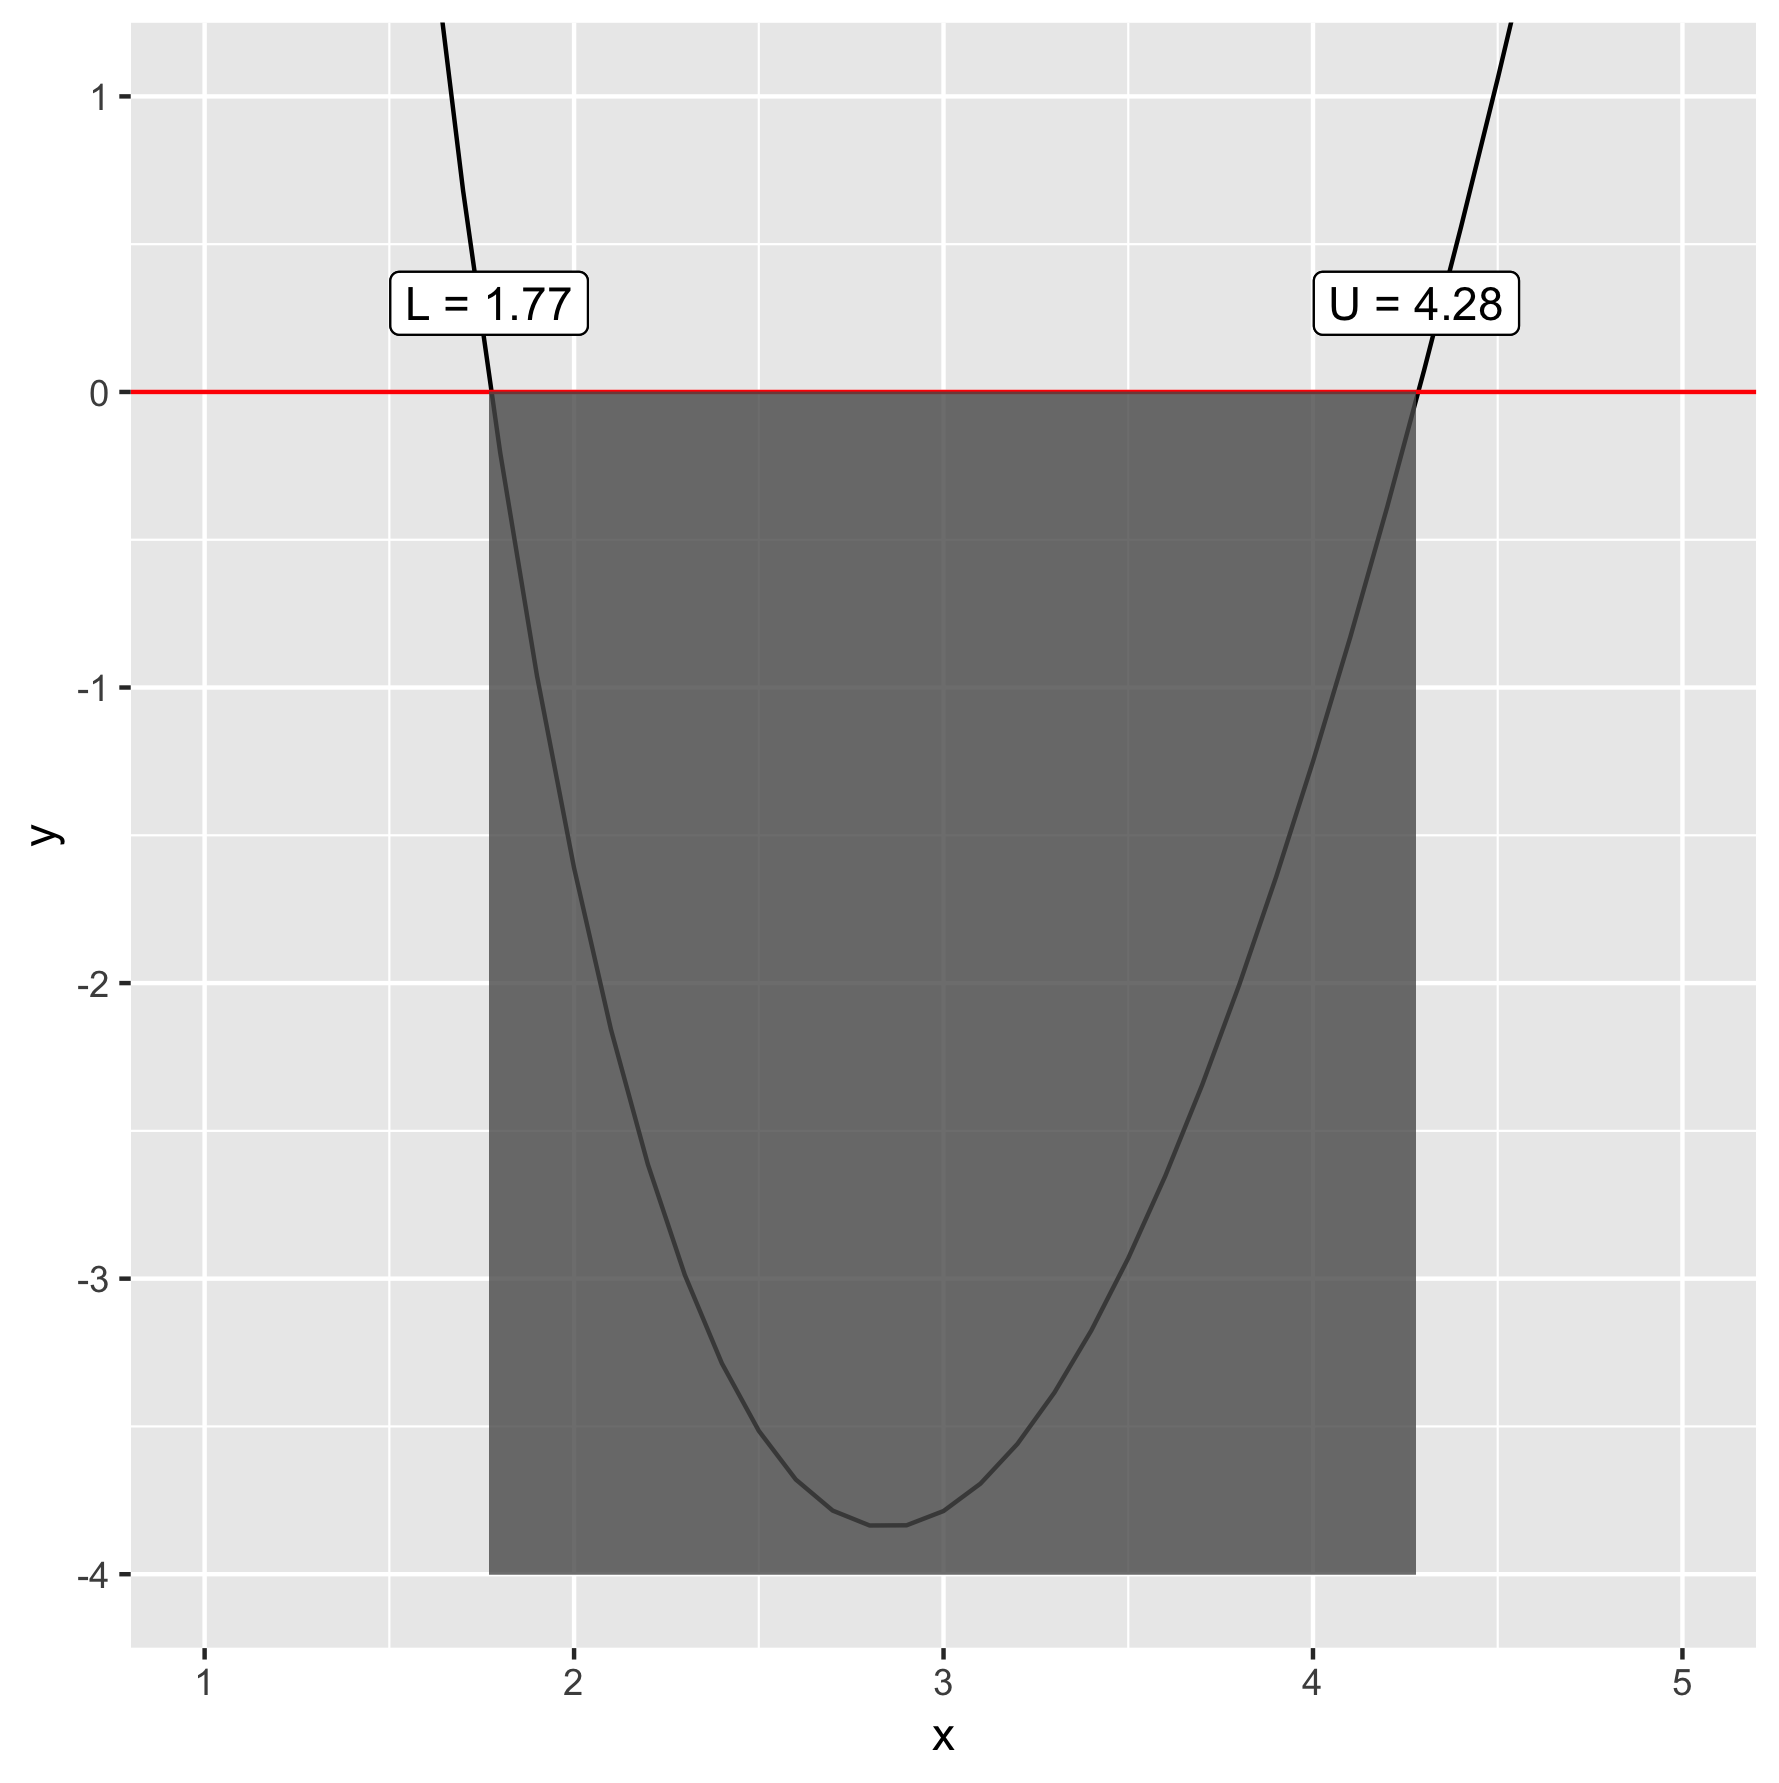
\includegraphics[scale=0.07]{src/ACT-2005/Q13-57_visualisation.png}
\end{center}

\section{Sélection de modèles}
\subsection*{Chi-Square \emph{Goodness-of-fit}}
On veut valider l'adéquation du modèle qu'on propose avec ce test. On calcule la quantité $X^2$ : 
\[X^2 = \frac{\sum_{j=1}^{k}(E_j - O_j)^2 }{E_j}\]
où $E_j = n \hat{p}_i$ est le nombre de valeurs qu'on s'attend à avoir dans la $i$\up{e} classe et $O_j = n p_{ni}$ le nombre d'observations dans la $i$\up{e} classe. On peut prouver que
\[X^2 \sim \chi_{k-p-1}^2\] \\

On peut aussi faire le test LRT pour valider l'adéquation aussi.

\subsection*{Critères de sélection}
Pour chosir entre plusieurs modèles, on peut, entre autres, se baser sur les critères suivants : 
\begin{enumerate}
\item la plus \textbf{faible valeur} pour le test \textbf{Kolmogorov-Smirnov} ; 
\item  la plus \textbf{faible valeur} pour le test \textbf{Anderson-Darling} ;
\item  la plus \textbf{faible valeur} pour le test \textbf{Goodness-of-fit} ;
\item la plus \textbf{haute valeur} pour la \textbf{\emph{p-value} du test Goodness-of-fit} ; 
\item la plus \textbf{haute valeur} pour la \textbf{fonction de vraisemblance à son maximum}.
\end{enumerate}

\section{Estimation bayésienne}
\begin{definition}[Distribution \emph{a priori}]
Soit un paramètre $\theta$ d'une distribution quelconque. Afin de réaliser une estimation Bayésienne, on connaît \emph{a priori} la distribution que prend le paramètre $\theta$, qu'on dénote par $\pi(\theta)$. \\

Alors, notre distribution des pertes est conditionnée par rapport à la valeur que $\theta$ prend (i.e. $f_{X|\Theta}$).
\end{definition}


\begin{definition}[Distribution \emph{a posteriori}]
La distribution \emph{a posteriori} nous permet de savoir avec quelle probabilité non-nulle notre paramètre $\theta$ peut prendre une certaine valeur, sachant qu'on a observé certains $x$, qu'on dénote comme $\pi_{\Theta | X}(\theta | x)$ : 
\begin{equation}
\label{eq:dist_posteriori}
\pi_{\Theta | X}(\theta | x) = \frac{f_{\Theta, X}(\theta, x)}{f_{X}(x)} = \frac{f_{X|\Theta}(x | \theta) \pi(\theta)}{\int f_{X|\Theta}(x | \theta) \pi(\theta) d \theta} 
\end{equation}
L'idée est de remplacer les différentes distributions dans l'\autoref{eq:dist_posteriori}, et en déduire une distribution avec une paramétrisation différente\footnote{Souvent, la distribution \emph{a posteriori} aura la même distribution que celle \emph{a priori}, mais avec des paramètres différents.}.
\end{definition}

\paragraph{L'estimateur Bayésien} L'estimateur Bayésien est défini comme l'espérance du paramètre $\theta$, sachant la distribution de $X$. En d'autres mots, on veut l'espérance de la distribution \emph{a posteriori} : 
\begin{equation}
\label{eq:estimateur_bayes}
\hat{\theta}_{BAYES} = \esp{\Theta | X}
\end{equation}

 \section{Rappel de probabilité}
 \subsection*{Certaines lois à savoir}
 \begin{tabular}{|a| * {4}{C|}}
 \hline
 \rowcolor{red!30!white}\text{Loi} & \prob{X = x} \text{ ou } f_X(x) & \esp{X} & Var(X) & M_X(t) \\\hline
 Bin(n,p)	& \binom{n}{x} p^x (1-p)^{n-x} & np & np(1-p) & \left( (1-p) + p^t \right)^n \\\hline
 Pois(\lambda) & \frac{e^{-\lambda} \lambda^x}{x!} & \lambda & \lambda & e^{\lambda(t-1)} \\\hline
 Gamma(\alpha, \lambda) & \frac{\lambda^{\alpha} x^{\alpha-1} e^{-\lambda x}}{\Gamma(\alpha)} & \frac{\alpha}{\lambda} & \frac{\alpha}{\lambda^2} & \left( \frac{\lambda}{\lambda - t} \right)^\alpha \\\hline
 Normale(\mu, \sigma^2) & \frac{1}{\sqrt{2 \pi} \sigma} e^{- \frac{1}{2} \left( \frac{x-\mu}{\sigma} \right)^2} & \mu & \sigma^2 & e^{\mu t + \frac{\sigma^2 t^2}{2}} \\\hline
 \end{tabular}
 
 \subsection*{Rappels d'algèbre linéaire}
\subsubsection*{Matrice transposée} la matrice transposée est définie par $\bm{A}^\top$, telle que
\begin{align*}
\bm{A}^{\top} & = 
\begin{bmatrix}
a	& -c \\
-b	& d \\
\end{bmatrix}
\end{align*}

\subsubsection*{Déterminant d'une matrice} On peut calculer le déterminant $\det(\bm{A})$ de la matrice $\bm{A}$ tel que
\begin{align*}
\det(\bm{A})	  = 
\begin{vmatrix}
a	& b \\
c	& d \\
\end{vmatrix}
= ad - bc
\end{align*}

\subsubsection*{Inverse d'une matrice} L'équivalent de l'opération $\frac{1}{\bm{A}}$ en algèbre linéaire est de calculer la matrice inverse de $\bm{A}^{-1}$, telle que
\begin{align*}
\bm{A}^{-1}	& = \frac{1}{\det(\bm{A})}
\begin{bmatrix}
a	& -c \\
-b	& d \\
\end{bmatrix}
\end{align*}
où on multiple par la matrice adjointe de $\bm{A}$. Il faut normalement calculer les cofacteurs, mais le cas à 2 dimensions est un cas simplifié.



\end{multicols*}


%% -----------------------------
%% Fin du document
%% -----------------------------
\end{document}
